% \documentclass[12pt]{article} \usepackage[letterpaper, margin=1in, %
%headheight=15pt]{geometry} \usepackage{amsmath, listings}


% \begin{document}
\section{Experiment 3.}

[I'm assuming Joe will include some preamble for the experiment, but otherwise
it should be fairly straightforward for me to churn out one anyway.]

\subsection{Participants, Materials, and Procedure}

Experiment 2 recruited 122 participants who each generated one set of four Alpha
and four Beta category exemplars. Among these 122 generated category sets were
102 unique sets (i.e., they contained a unique collection of Alpha and Beta
exemplars). Consequently, for Experiment 3, we recruited 102 participants with
one participant presented with a different unique category set.

Participants observed four blocks of eight trials. Each trial began with the
presentation of a fixation cross for 500 ms. This was followed by the
presentation of one exemplar randomly sampled without replacement from the
unique category set. Participants were tasked with assigning the presented
exemplar to either the Alpha or Beta category with no time limit imposed.
Feedback was automatically displayed for 2500 ms after each response.

\subsection{Results}

Overall accuracy of the participants was high, with a mean error rate of $.19$
($SD = .19$). Error rates for each block are presented in Figure
\ref{fig:learningcurve}. 

\begin{figure}
    \begin{center}
    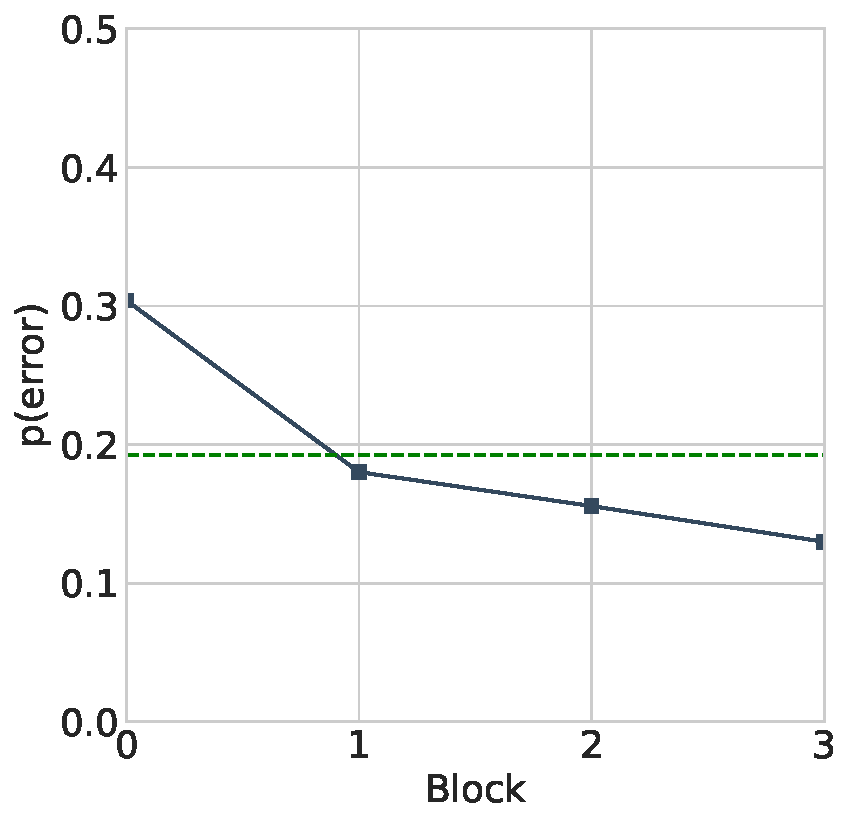
\includegraphics[width=\textwidth/2]{figs/e3-learningcurve.pdf}
    \caption{Average error rate for each successive block. Green discontinuous
      line represents the overall mean error rate.}
    \label{fig:learningcurve}
    \end{center}
\end{figure}

In the previous section (or Section X.X), we demonstrated that the best
performing models were the two contrast models. In this section, our goal is to
investigate if contrast is also important in category learning tasks.

It is also the
goal of this paper to demonstrate that there is an association between the
model's [justifying the errorvscat plot is harder than I thought] To compare the
performances of each model, we analysed the correlation between each model's fit
to a participant's unique category set and the participant's error rate.
Intuitively, a well-performing model should be able to closely fit (i.e., easily
generate) A positive correlation would indicate that the model is We used the
same set of optimised parameters found from Section X.X, with individual values
for selective attention.

\begin{figure}
    \begin{center}
    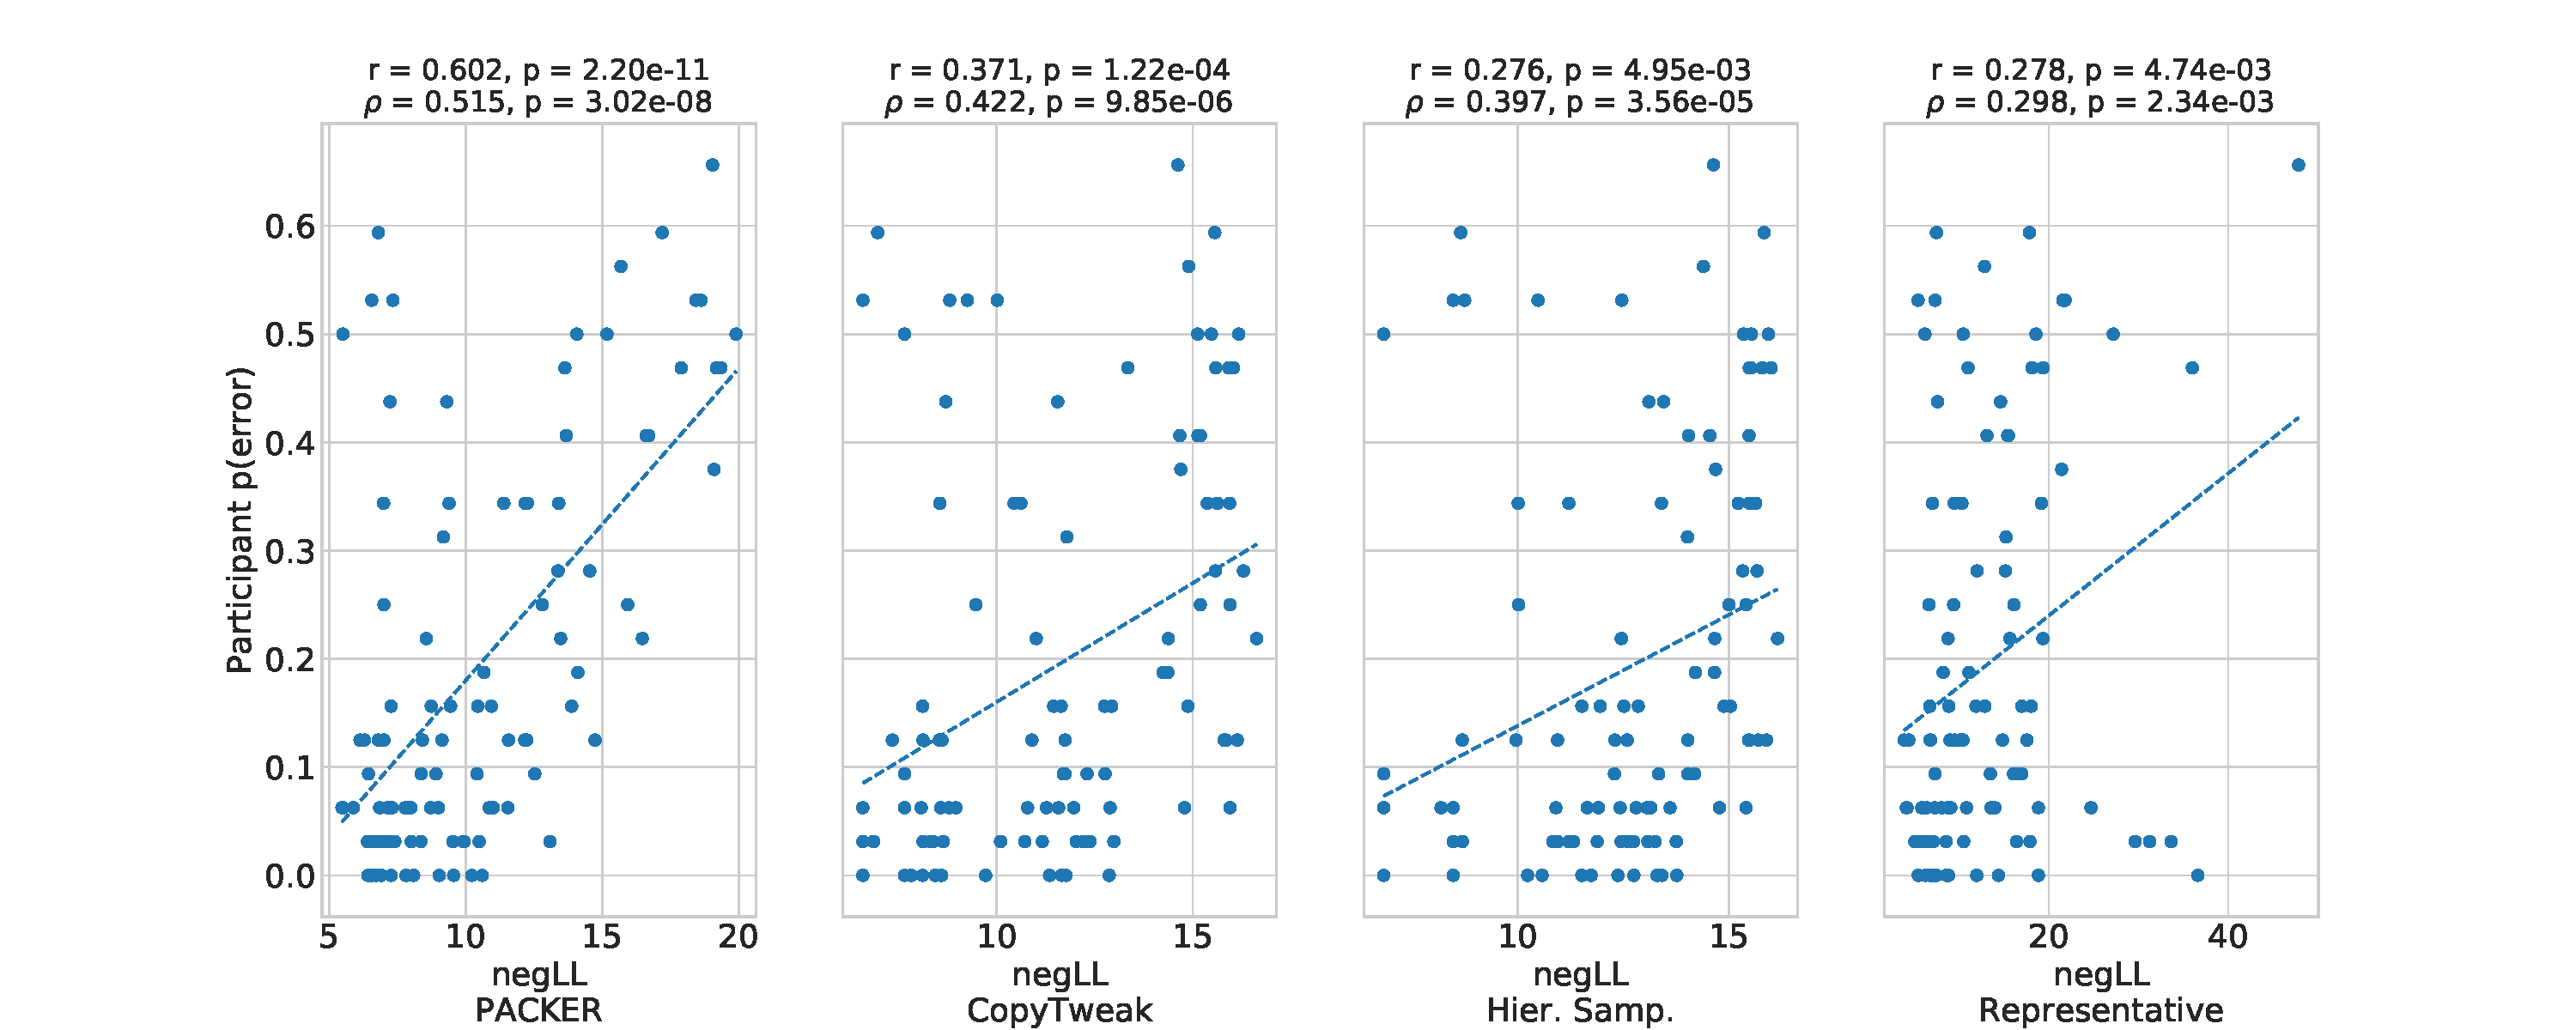
\includegraphics[width=\textwidth]{figs/perror_corr.pdf}
    \caption{Correlation between observed participant error and model fit.}
    \label{fig:perror_corr}
    \end{center}
\end{figure}

To emphasize the strong influence of contrast in maximizing the association
between category generation and category learning, we computed the correlations
over wide range of $\theta_{contrast}$ values, with the other parameter values of
PACKER held constant at their optimized levels. As presented in Figure
\ref{fig:packer-corr}, the correlation quickly increases with increasing weight
on contrast, reaching a plateau above values of around 4.0.

\begin{figure}
    \begin{center}
    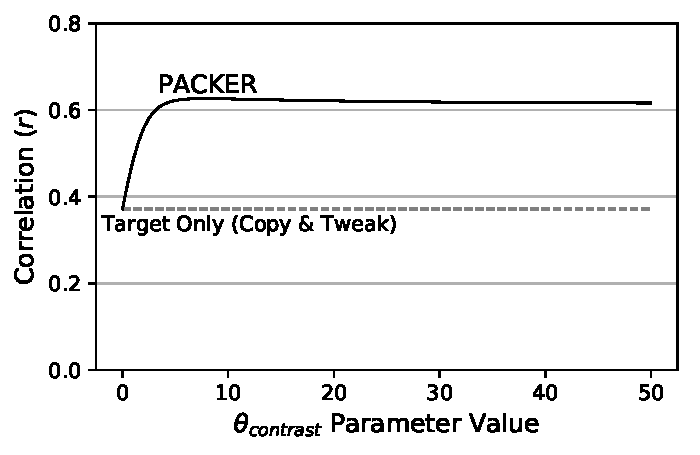
\includegraphics[width=0.8\textwidth]{figs/packer-corr.pdf}
    \caption{Correlation between PACKER's fit and participant error as a
      function of the $\theta_{contrast}$ parameter. To facilitate comparison,
      PACKER's other parameters ($c$, $\theta_{target}$) were set to the best
      fitting values obtained for copy-and-tweak in Table
      \ref{table:global-model-fits}. Grey dashed line represents the correlation
      between Copy \& Tweak's fit and participant error.}
    \label{fig:packer-corr}
    \end{center}
\end{figure}


The specific reason for why contrast as implemented in PACKER is superior to
contrast as implemented in the representativeness model is still not clear.

[Note Joe's comments on figure formatting (font size, remove redundant y-axes,
etc)]













